\documentclass[12pt,a4paper]{amsart}
%\usepackage[norsk]{babel}
\usepackage[english]{babel}
\usepackage[utf8]{inputenc}
%\usepackage[fleqn]{amsmath}
\usepackage{amsmath}
\usepackage[T1]{fontenc}
\usepackage{mathtools}
\usepackage{graphicx}
\usepackage{subcaption}
\usepackage{verbatim}
\usepackage{listings}
\usepackage{scalerel}
\usepackage{fixltx2e}
\usepackage{amssymb}
\usepackage{siunitx}
\usepackage{xfrac}
\usepackage{enumitem}
\usepackage{hyperref}
\usepackage{float}
\usepackage{bbold}
\usepackage{physics}
\usepackage[ampersand]{easylist}
\usepackage{subcaption}
\usepackage{wrapfig}
\usepackage{algorithmicx}
\usepackage{csquotes}
\usepackage{xcolor}

%%For visualizations of table
\usepackage{multirow}
\usepackage{arydshln}
\usepackage{booktabs}

\usepackage[english]{babel}\addto\captionsenglish  
{\renewcommand{\bibname}{References}}  
\usepackage[backend=bibtex,style=phys]{biblatex}  %backend=biber is 'better'  
%\usepackage[backend=biber]{biblatex}
%\usepackage{apacite}
\addbibresource{cosmic_rays_bibliography.bib}

\usepackage[margin=1.5in]{geometry}
\newcommand{\scalel}{\scaleleft{<}}
\newcommand{\scaler}{\scaleright{>}}

%% physics packages
\usepackage{physics}
\usepackage[compat=1.1.0]{tikz-feynman}
\usepackage{feynmf}

% adjust the spacing around figure if pdf-file with white space:
\usepackage[font=small,skip=0pt]{caption}
%\usepackage[margin=1.4in]{geometry}
%\captionsetup[figure]{skip=-100pt}

% define colors for text
\definecolor{mygreen}{RGB}{28,172,0} % color values Red, Green, Blue
\definecolor{mylilas}{RGB}{170,55,241}
\definecolor{forestgreen}{rgb}{0.13, 0.55, 0.13}

% definitions of commands
\renewcommand{\thesection}{\arabic{section}}
\newcommand{\M}{\CMcal{M}}
\newcommand{\p}[1]{p_{#1}}  %p with one parameters such that \p1 = p_1, \p2 = p_2 etc.
\newcommand{\q}[2]{\ensuremath{p_{#1}\cdot p_{#2}}}  %p with two parameters such that \p12 = p_1\cdot p_2
\newcommand{\cmuplus}{c_V^2 + c_A^2}
\newcommand{\cmuminus}{c_V^2 - c_A^2}
\newcommand{\cbplus}{\tilde{c}_V^2 + \tilde{c}_A^2}
\newcommand{\cbminus}{\tilde{c}_V^2 - \tilde{c}_A^2}

% layout for sections, subsections and subsubsections
\usepackage{titlesec}
\renewcommand{\thesubsection}{\arabic{subsection}} % Arabic numerals for the subsections
\renewcommand{\thesubsubsection}{\arabic{subsubsection}} % Arabic numerals for the subsections
\titleformat{\subsection}{\scshape\large\filcenter}{\arabic{section}.\thesubsection}{1em}{}
\titleformat{\subsubsection}{\scshape\normalsize\filcenter}{\arabic{section}.\thesubsection.\thesubsubsection}{1em}{}

\title[Charged particles study with PolarquEEEst]{Project 2: \\Study of cosmic charged particle events with the PolarquEEEst experiment\\
\small{\mdseries FYS5555 - Spring 2020}}
\date{\today}
\author[Christensen]{Elisabeth Christensen}

\begin{document}
\maketitle
\setcounter{section}{1}
\setcounter{subsection}{0}
\subsection{Cosmic Rays}
The study of cosmic rays began in the beginning of the 20'th century, and was triggered by the fact that radiation was able to penetrate even those of the most isolating materials. Using electrometers, one could measure the intensity of radiation at different altitudes. In 1912, Victor Hess discovered~\cite{Hess1912} that the radiation increased with increasing altitudes, meaning that the radiation must originate beyond our atmosphere. He excluded the Sun as the sole source of this type of radiation, and concluded that it can also come from more distant sources such as other galaxies. Now, the reason as to why we wish to know more about these cosmic rays is due to their astonishingly high energies. An example of this is the 'Oh-My-God' particle, measured by the Fly's Eye experiment~\cite{OhMyGodParticle}, which reached the Earth's surface with an energy of $3.2\cdot 10^{20}$eV, i.e. more than a billion times greater than what our most advanced accelerators to date can manage. This leaves us with the bigger questions to answer. Where do these particles come from and how did they reach such high energies?

Primary cosmic rays are essentially high-energetic protons and alpha particles originating from the Sun or beyond our Solar system. Models indicate that cosmic rays of energies up to $\sim 10^{15}$eV originate from the shock fronts of supernova remnants~\cite{Ellison1997}. The AGASA observatory, situated in Japan, measures the higher end of the energy spectrum, i.e. up to $10^{20}$eV, of cosmic rays entering our atmosphere. Another observatory, the Pierre Auger Observatory, published its first results of the highest-energy cosmic rays in 2007. The observatory has also assisted in finding the energy spectrum for cosmic rays above $\sim 10^{18}$eV~\cite{Auger2010}, and found that the flux was propotional to $E^{-\gamma}$, where $\gamma$ is approximately equal to 3. It also supported the theory that within the center of each galaxy resides a black hole with the capacity to accelerate particles to energies up to $10^{20}$eV.

Secondary cosmic rays are essentially particle showers occuring when the primary cosmic rays interact with particles within our atmosphere. These cosmic rays typically consist of neutrons and charged mesons which subsequently can decay to muons and neutrinos reaching the Earth's surface. There are many experiments dedicated to use secondary cosmic particles in the search for knowledge. Some examples are the CLOUD experiment at CERN~\cite{cloud2000}, designed to measure the correlation between cosmic rays and cloud formation, the balloon-borne experiment TRACER~\cite{tracer2007} designed to observe cosmic-ray nuclei at high energies, and the ground-based Cherenkov Telescope Array (CTA) observatory~\cite{cta2011}, dedicated to find the origin and role of relativistiv cosmic particles through the study of high-energy gamma-rays reaching Earth.

\setcounter{section}{2}
\setcounter{subsection}{0}
\subsection{POLA Detectors}
Particles can be detected in numerous ways depending on their charge and energy, some examples being the ionization chamber, the proportional counter and the Geiger-Müller counter. The Geiger-Müller counter was one of the first few devices to detect particles and consists simply of an air-tight cylinder tube containing a suitable gas and a suspended conducting wire with a positive voltage. When charged particles strike the gas they interact with molecules within the gas creating electron-ion pairs. The electrons will be accelerated towards the conducting wire, i.e. the anode, whereas ions will be accelerated towards the cathode. The total eletron-ion pairs collected results in a measurable electric current. Another example is that of scintillators.

Scintillators are based on the principle of luminescense~\cite{knoll2000}. In other words, as passing radiation strikes a luminescent material it converts the kinetic energy of the charged particles to detectable light. Put simply, scintillators gather the information of the emitted photons in photomultiplier tubes which outputs a current of electrons based on the energy of the impinging photon.

\begin{comment}
The PolarquEEEst experiment~\cite{PolarquEEEst_first_results} consists in total of three POLA detectors, each with the aim to measure the intensity of incoming atmopheric radiation at a certain latitude. POLA-01 was placed upon an 18m long boat, known as \textit{Nanuq}, and was shipped from Isafjord, Iceland to Tromsø, Norway continuously taking measurements between the latitudes of $66^\circ-82^\circ$N. POLA-03 is situated in Bra, Italy at a latitude of $44^\circ 41'$N, while POLA-02 is situated in Nesodden, Norway at a latitude of $59^\circ 51'$N.  The two latter detectors were used as references. POLA-01 also performed measurements down to $35^\circ$ in Italy at a later point in time.
\end{comment}

Each of the POLA detectors consists of two floors of four plastic scintillators with the dimensions $20\times30\times1 \si{cm}^3$. The main purpose of a plastic scintillator is to emit photons within the energy range of any passing charged particle. Plastic scintillators can provide an extremely fast signal with a decay constant of about 2-3$\si{ns}$ along with a high light output~\cite{leo1994}. Attached to each scintillator is a pair of silicon photomultiplier (SiPM) tubes. Included are also eight front-end boards each dedicated to handle the SiPM signals separately, and trigger on events with a $10$ns resolution.

\setcounter{section}{3}
\setcounter{subsection}{0}
\subsection{Environmental Conditions}
From figure~\ref{fig:indoortemp_POLA-01} we can see the variations in indoor temperature onboard the 18m long sailboat Nanuq containing the detector POLA-01, from 22'nd of July 2018 to 4'th of September 2018. Each point represents the average indoor temperature recorded per event over a time interval of 10 minutes. The corresponding indoor temperatures for POLA-02 and POLA-03 can be seen in figures~\ref{fig:indoortemp_POLA-02} and~\ref{fig:indoortemp_POLA-03}. Figure~\ref{fig:outdoortemp} shows the temperatures close to the electronics for each detector. The corresponding mean values and sample standard deviations of the temperatures can be seen in table~\ref{tab:temperatures}. Here, we see that the variations in temperature for POLA-01 are much greater than that for POLA-02 and POLA-03, which can be explained by the fact that it was subject to varying weather conditions while travelling between Isafjord, Iceland and Tromsø, Norway.

Figure~\ref{fig:pressure} shows the atmospheric pressure each detector is subject to. This is dependent on the surrounding temperature and the elevation above sea level. As can be seen for POLA-03, situated in Bra, Italy, the pressure remains lower due to its elevation of approximately 278m above sea level. The effects of elevation can also be seen for POLA-02, situated in Nesodden, Norway at 81m, and POLA-01 onboard the sailboat Nanuq, which are subjects to a higher overall atmospheric pressure than that of POLA-03. The fluctuations of the atmospheric pressure arises due to the variations in temperature. One can see that the pressure resembles the patterns of temperature in figures~\ref{fig:indoortemp} and~\ref{fig:outdoortemp}.


\begin{table}[t]
\caption{Mean values of indoor, $\mu_{T, in}$, and outdoor, $\mu_{T, out}$, temperatures of each detector.}
\label{tab:temperatures}
\begin{tabular}{c|cc}
\hline
\hline
        & $\mu_{T, in} ({}^\circ \si{C})$ &$\mu_{T, out}({}^\circ \si{C})$ \\ \hline
POLA-01 & $25.39\pm 2.79$	& $23.75\pm 2.73$ \\
POLA-02 & $25.06\pm 0.14$    & $24.13\pm 0.12$ \\
POLA-03 & $33.37\pm 0.85$    & $34.67\pm 0.75$ \\
\hline \hline
\end{tabular}
\end{table}

\begin{figure}
\centering
	\begin{subfigure}[b]{\textwidth}
	\centering
		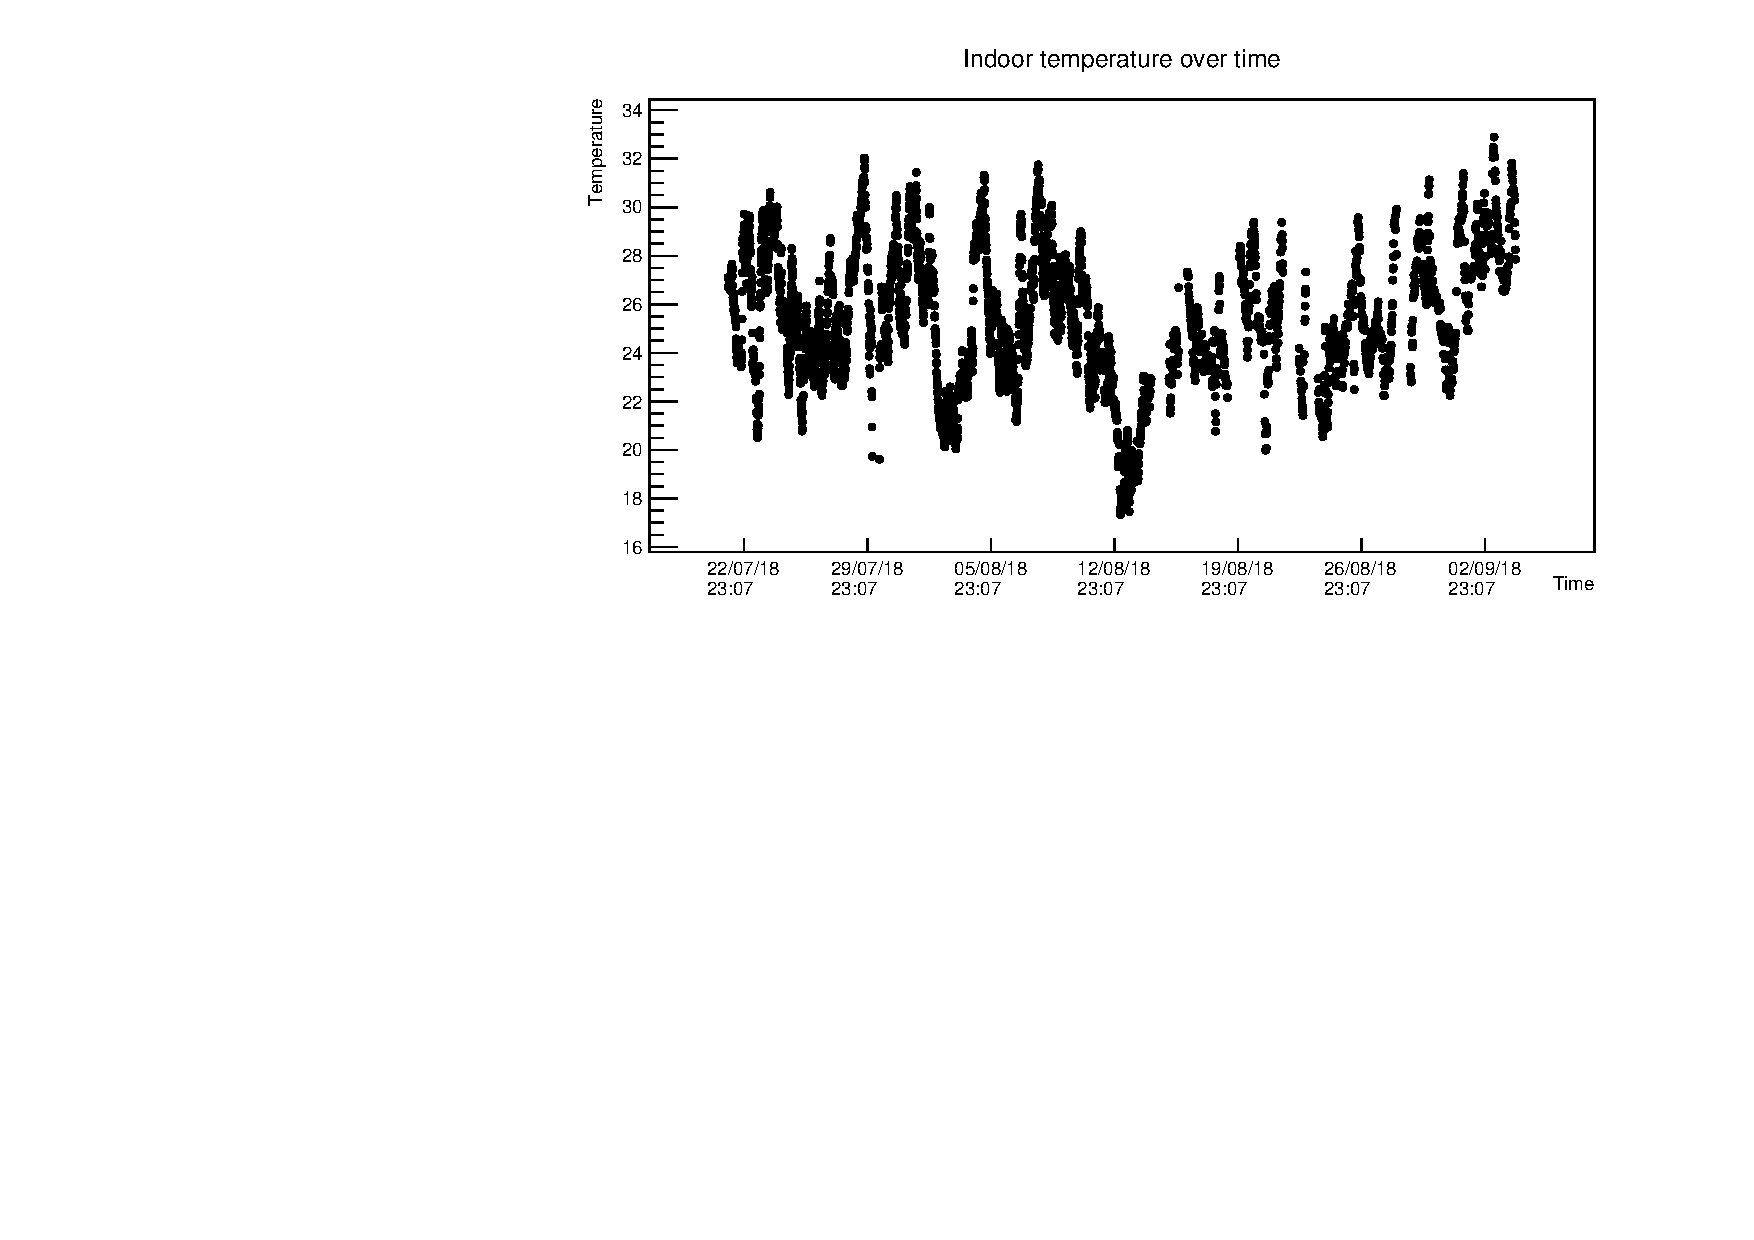
\includegraphics[width=\textwidth]{../data/plots/POLA-01/IndoorTemp_POLA-01.pdf}
		\caption{POLA-01}
		\label{fig:indoortemp_POLA-01}
	\end{subfigure}
	
	\begin{subfigure}[b]{0.6\textwidth}
	\centering
		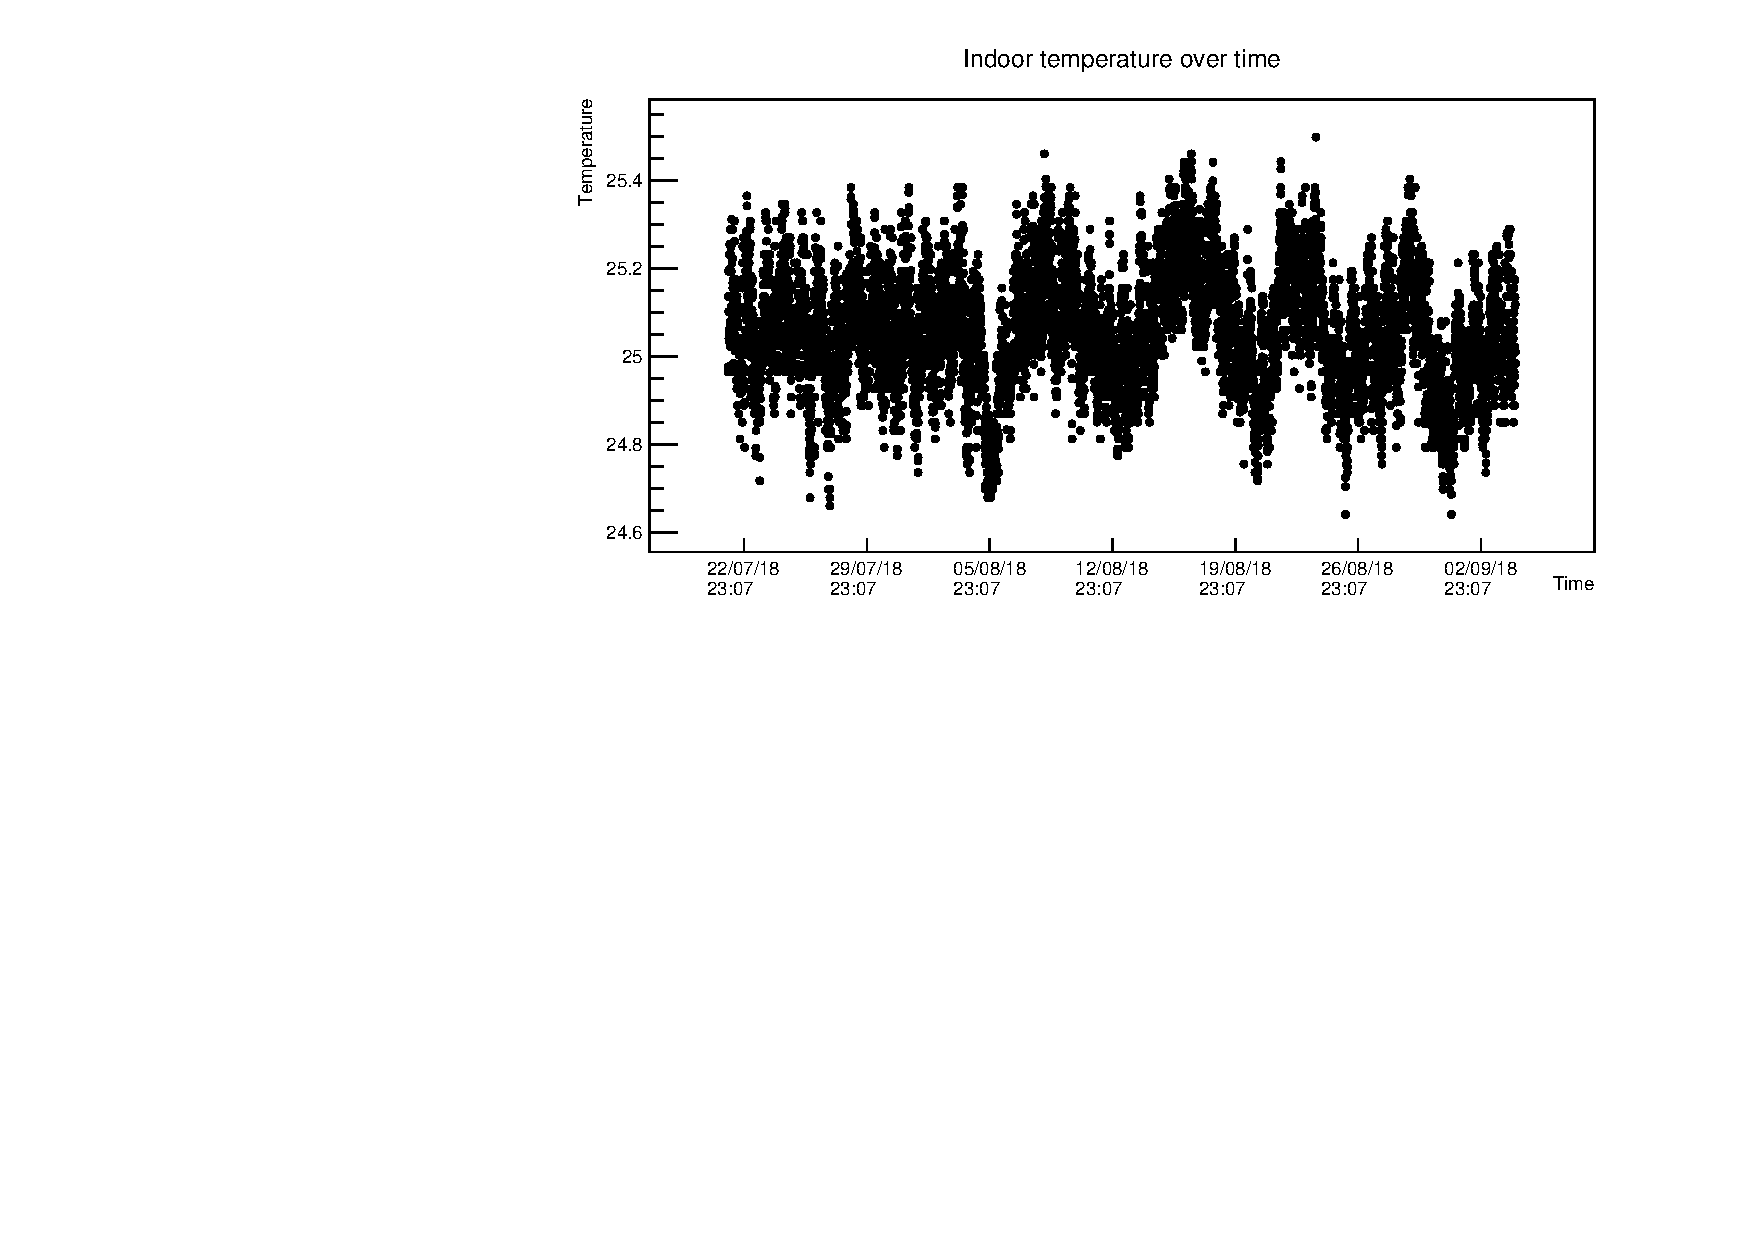
\includegraphics[width=\textwidth]{../data/plots/POLA-02/IndoorTemp_POLA-02.pdf}
		\caption{POLA-02}
		\label{fig:indoortemp_POLA-02}
	\end{subfigure}%
	\begin{subfigure}[b]{0.6\textwidth}
	\centering
		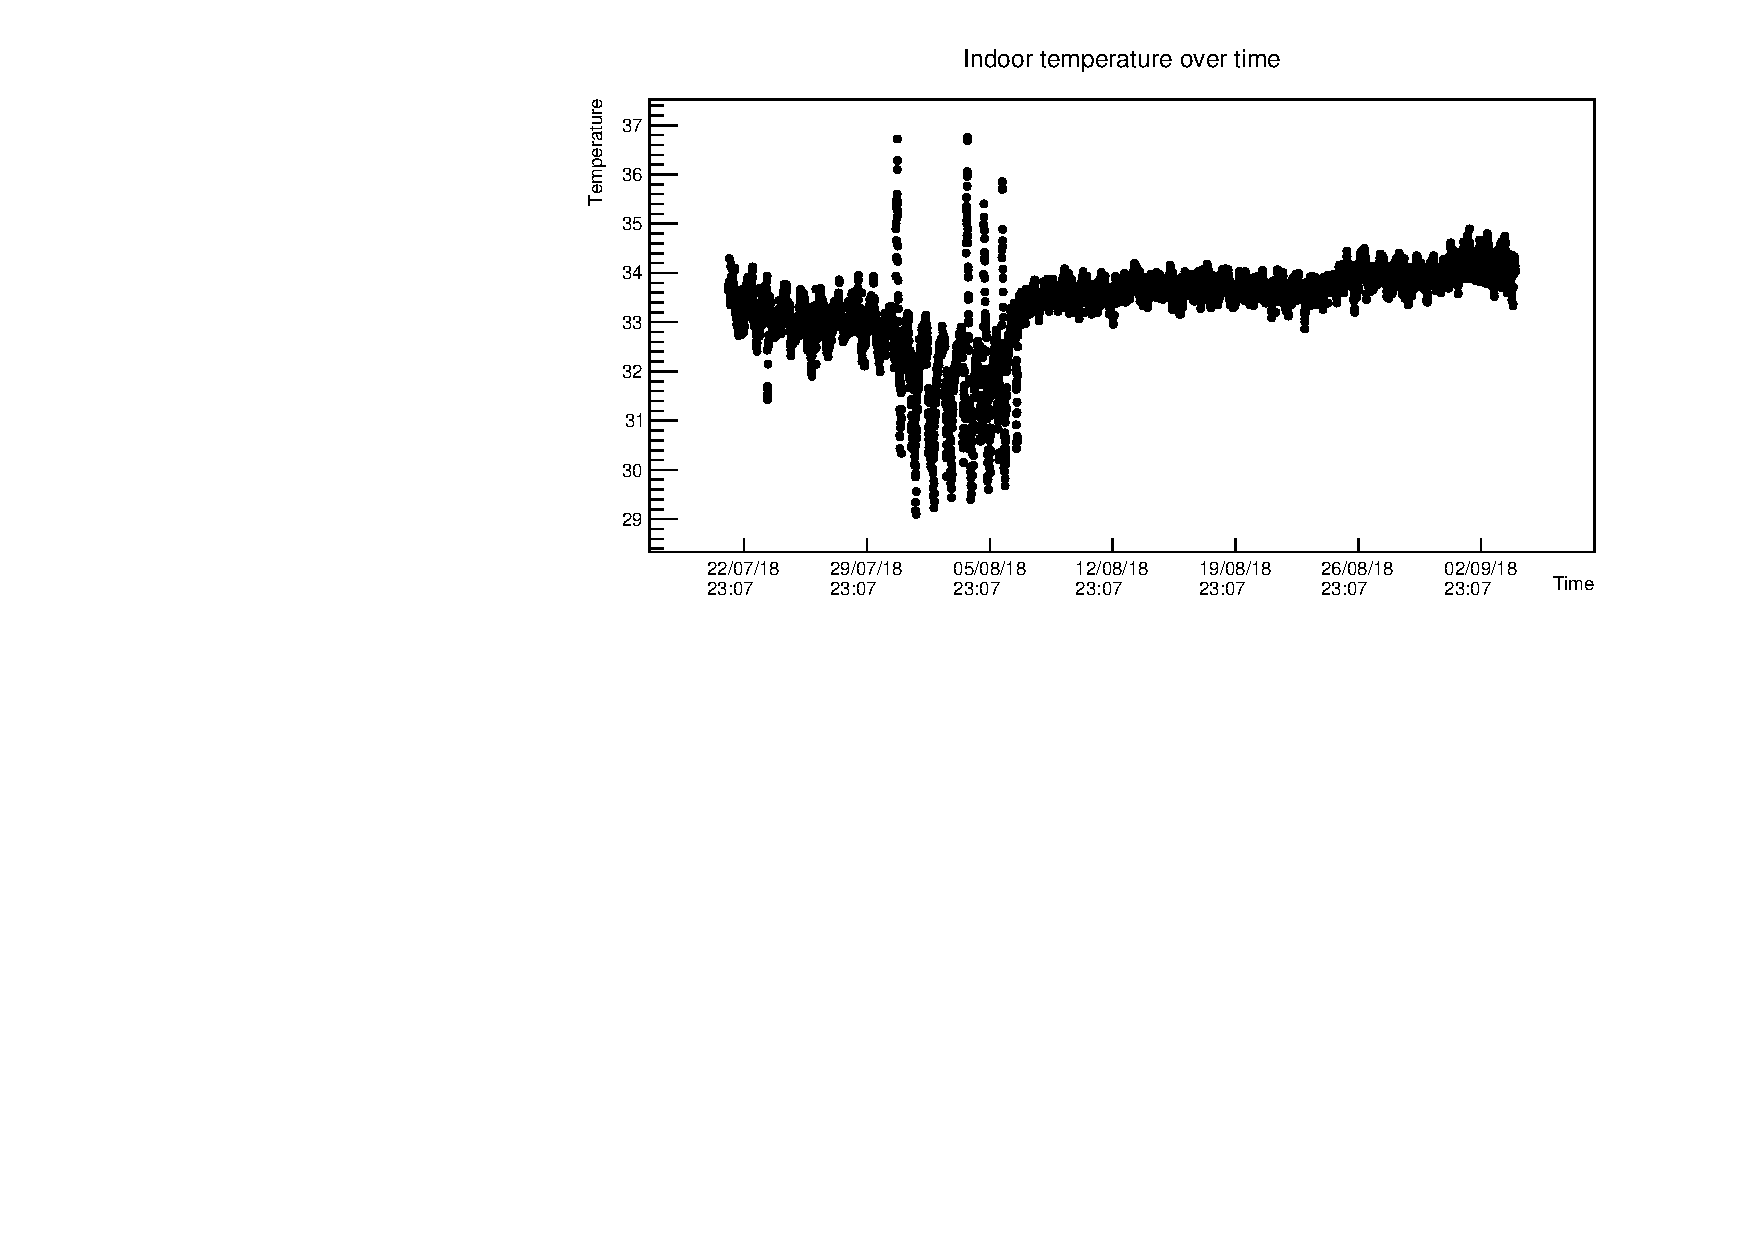
\includegraphics[width=\textwidth]{../data/plots/POLA-03/IndoorTemp_POLA-03.pdf}
		\caption{POLA-03}
		\label{fig:indoortemp_POLA-03}
	\end{subfigure}
	\caption{Indoor temperature as measured within each room containing the detectors.}
	\label{fig:indoortemp}
\end{figure}

\begin{figure}
\centering
	\begin{subfigure}[b]{\textwidth}
	\centering
		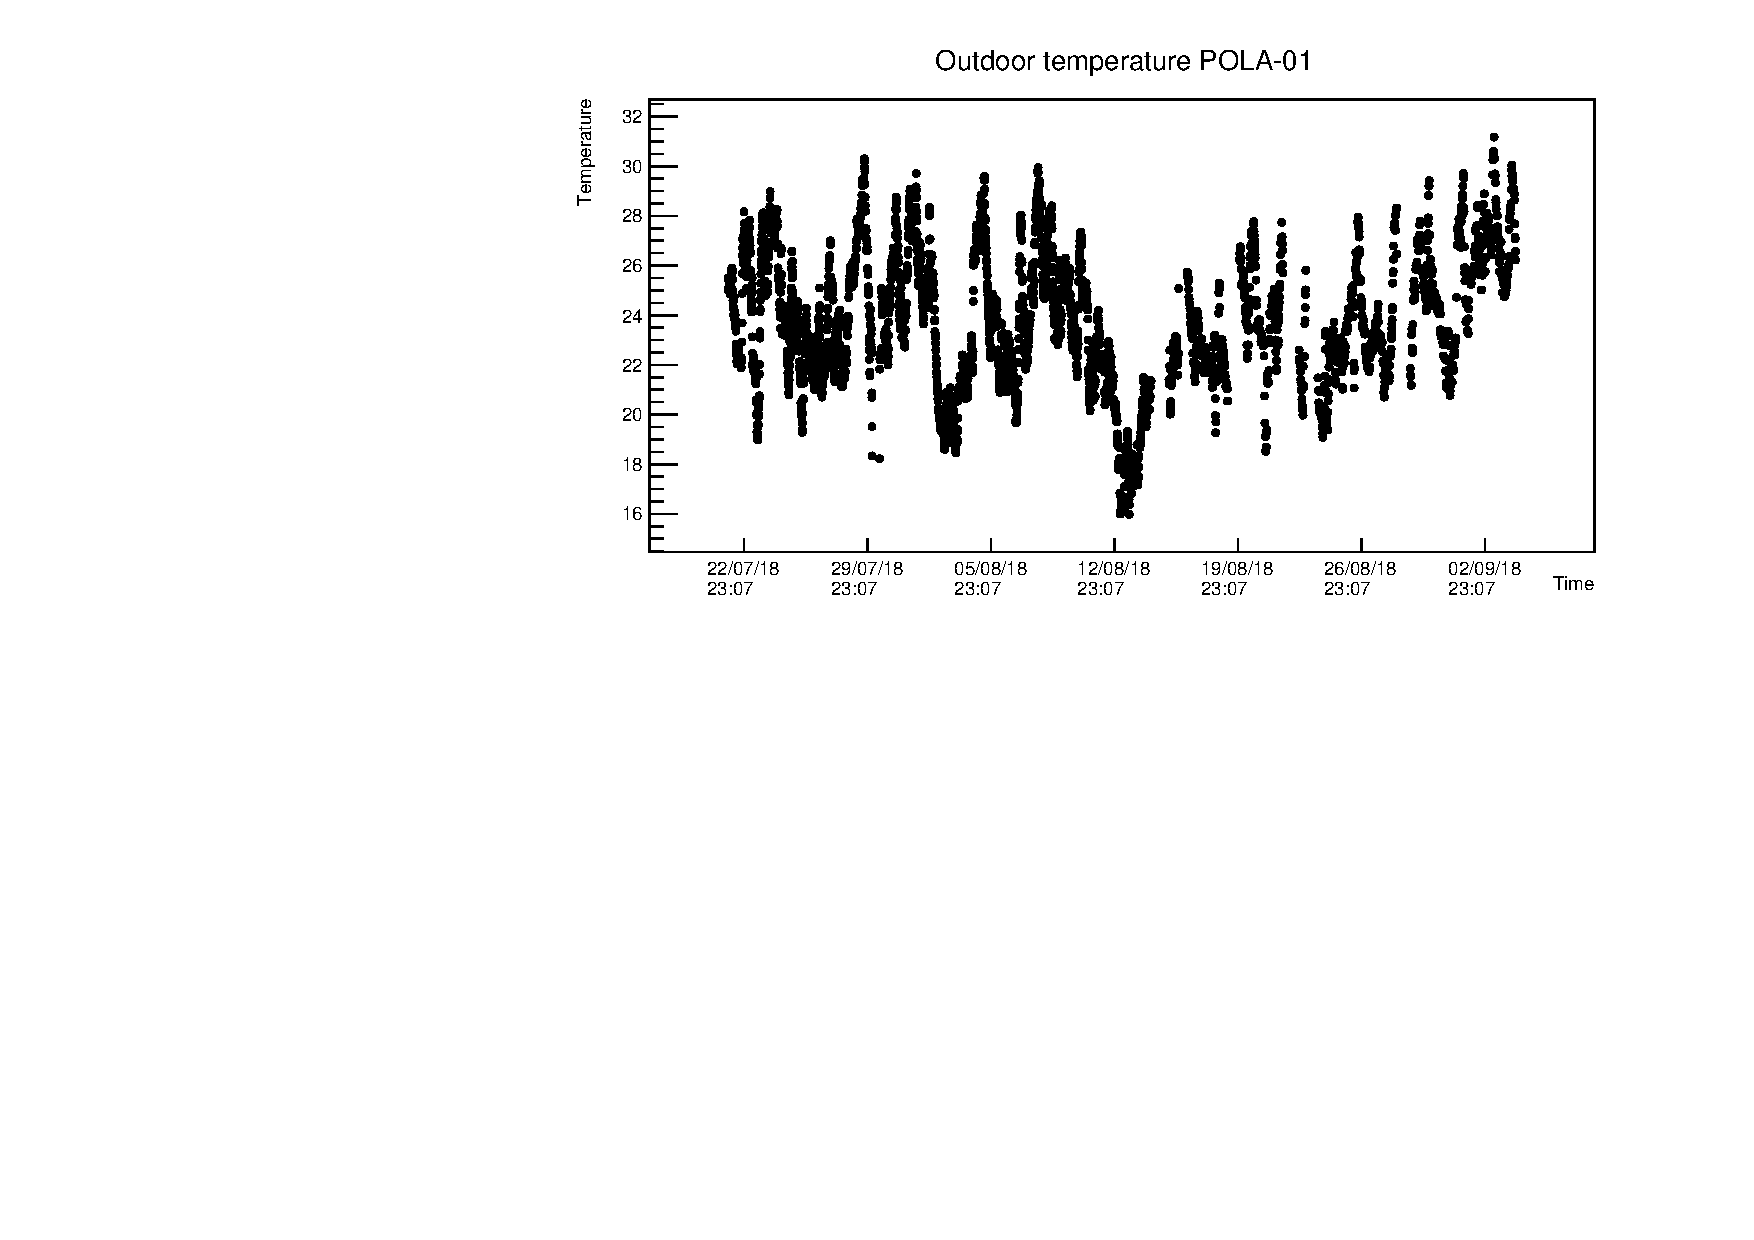
\includegraphics[width=\textwidth]{../data/plots/POLA-01/OutdoorTemp_POLA-01.pdf}
		\caption{POLA-01}
		\label{fig:outdoortemp_POLA-01}
	\end{subfigure}
	\begin{subfigure}[b]{0.6\textwidth}
	\centering
		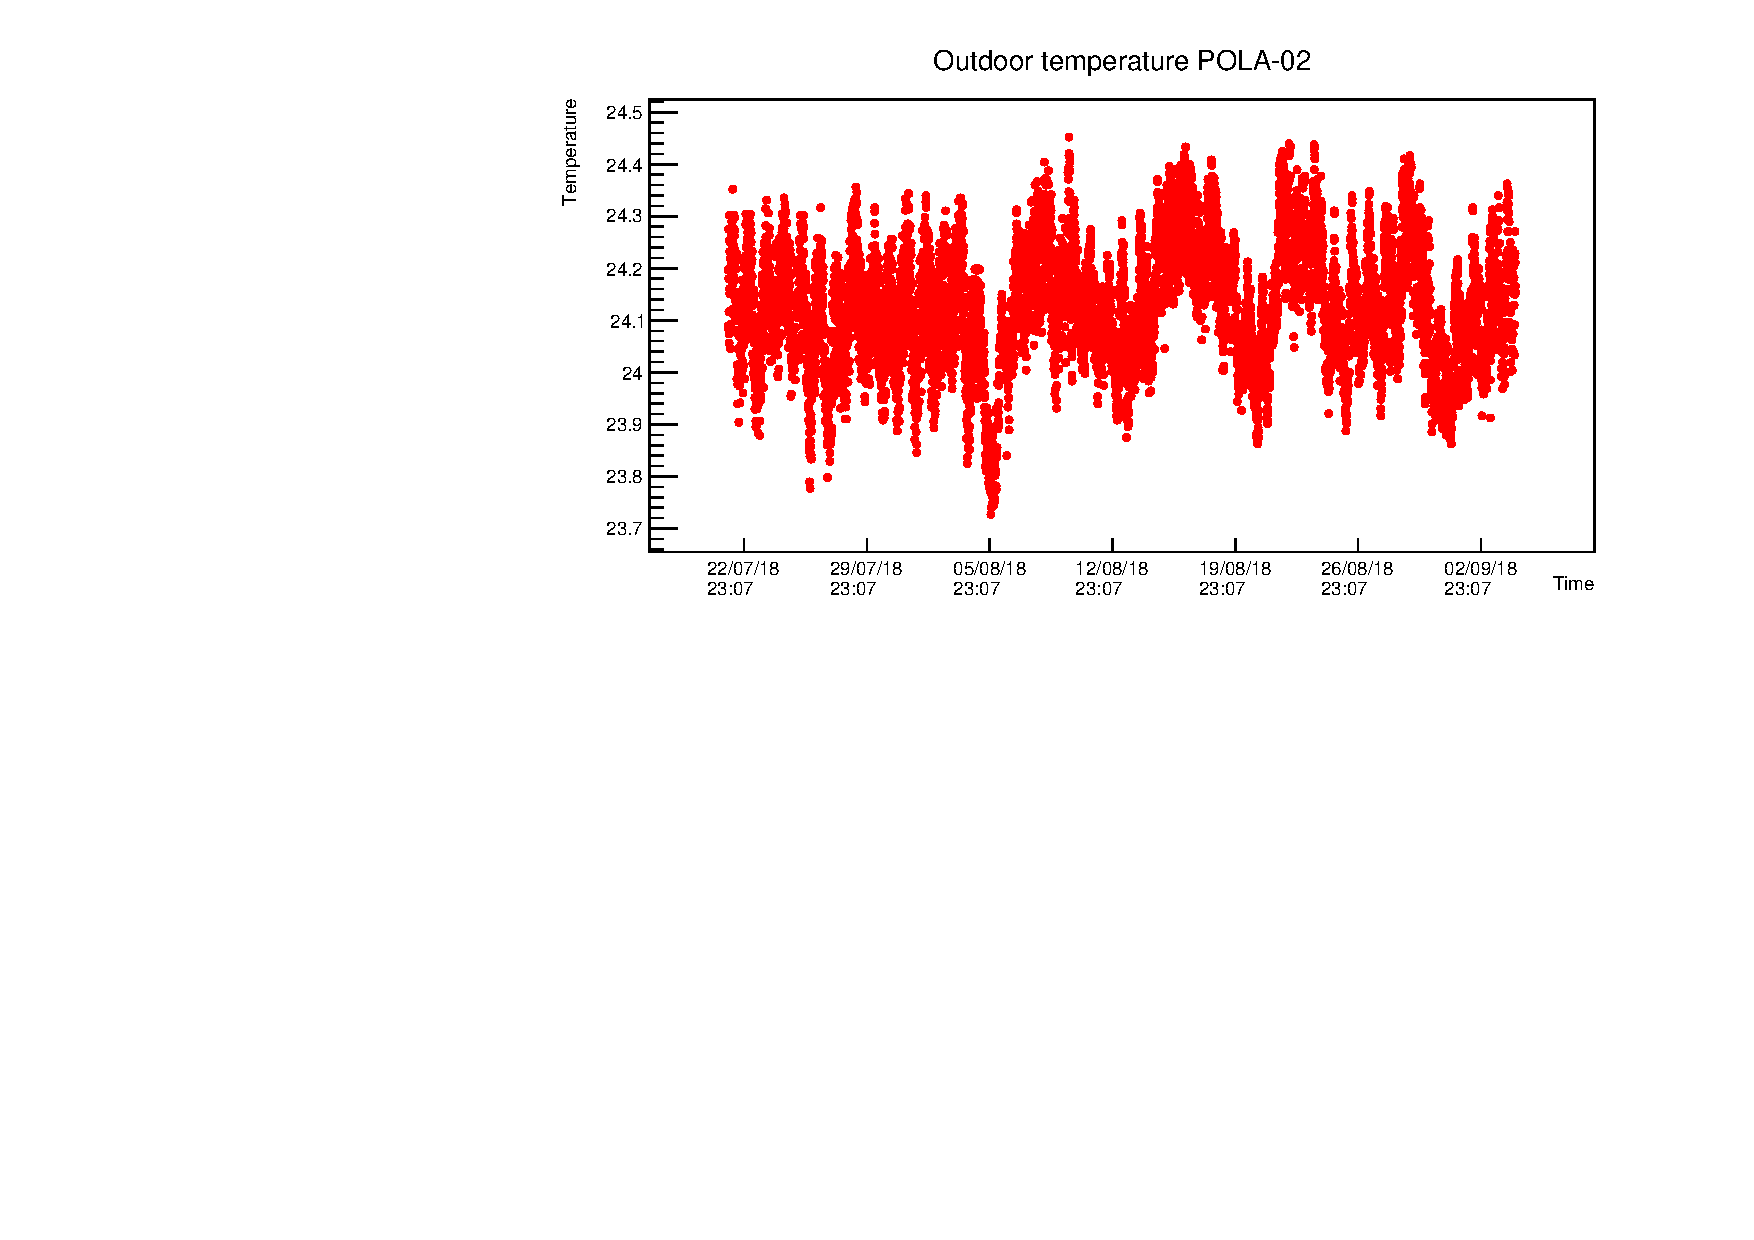
\includegraphics[width=\textwidth]{../data/plots/POLA-02/OutdoorTemp_POLA-02.pdf}
		\caption{POLA-02}
		\label{fig:outdoortemp_POLA-02}
	\end{subfigure}%
	\begin{subfigure}[b]{0.6\textwidth}
	\centering
		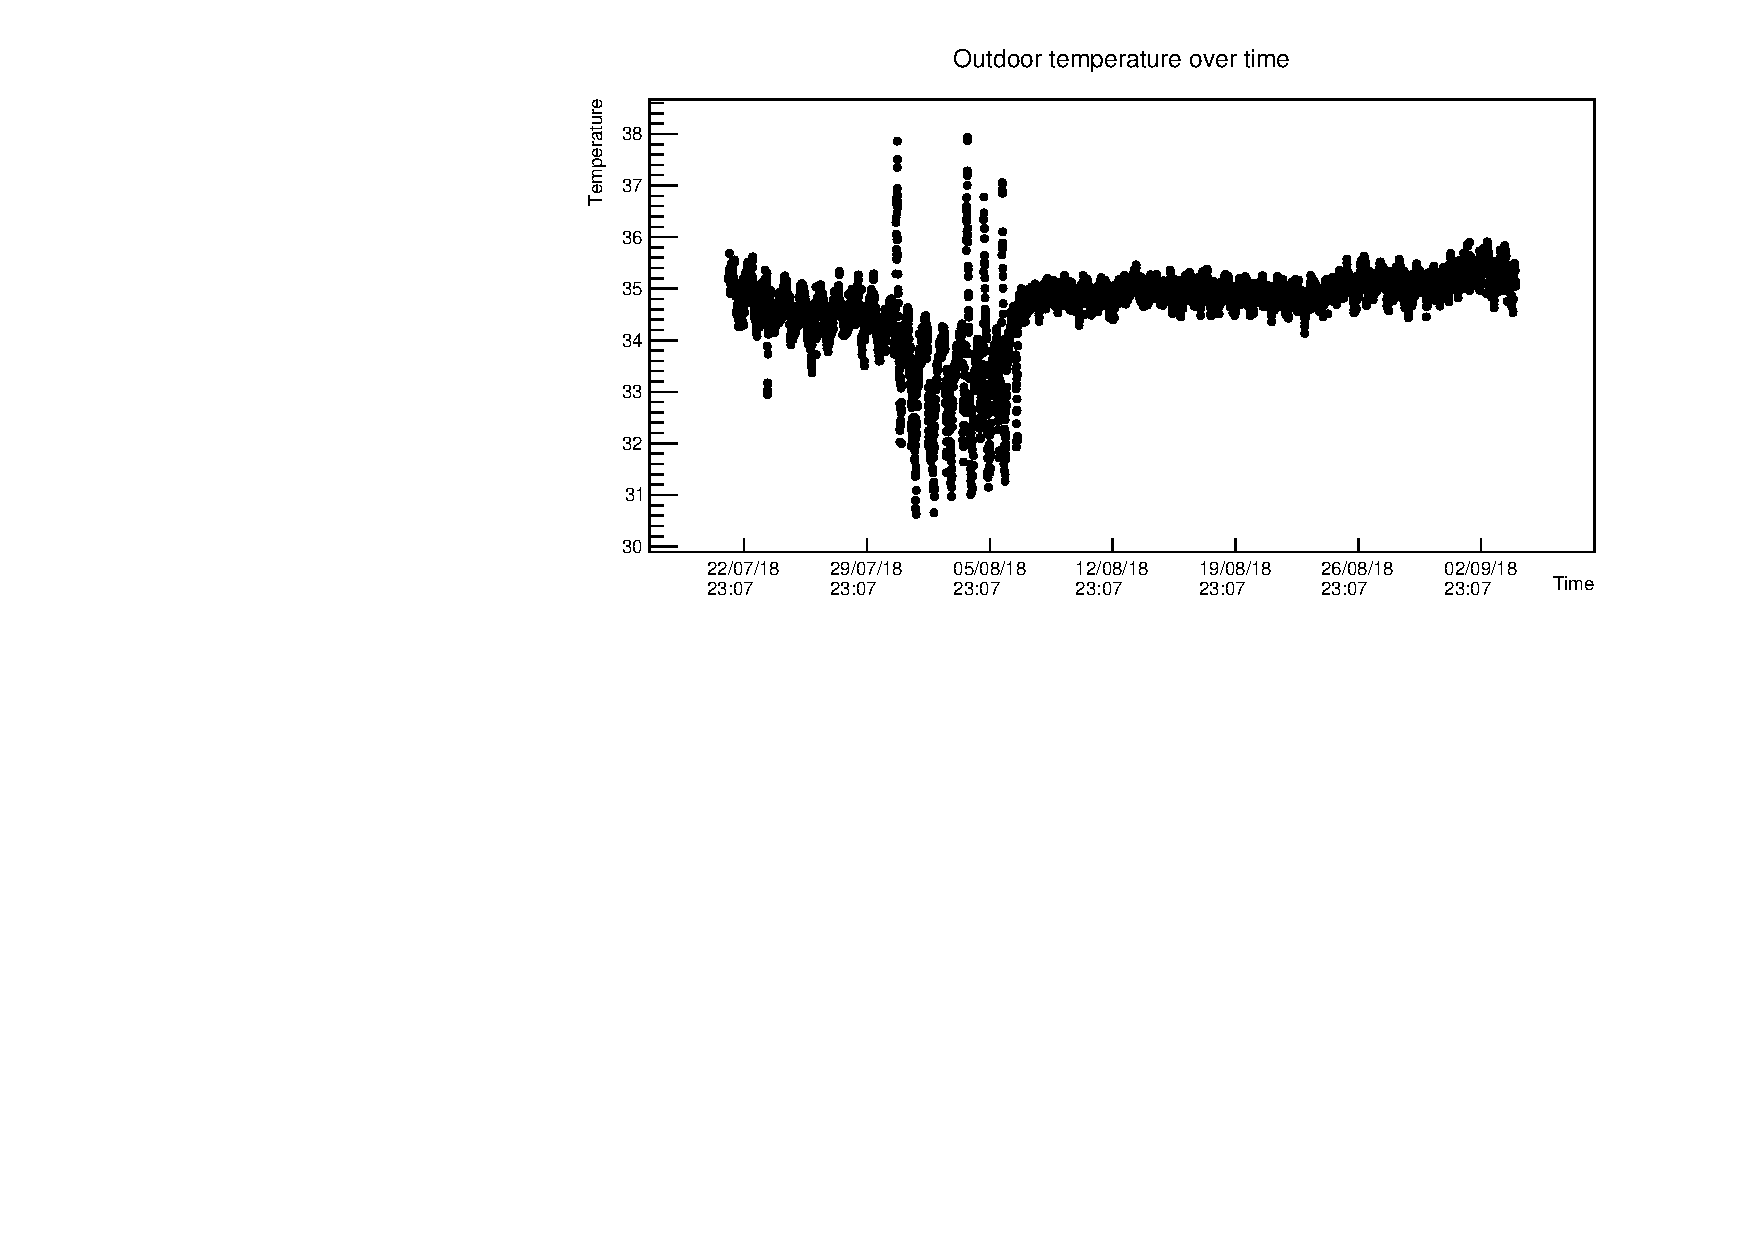
\includegraphics[width=\textwidth]{../data/plots/POLA-03/OutdoorTemp_POLA-03.pdf}
		\caption{POLA-03}
		\label{fig:outdoortemp_POLA-03}
	\end{subfigure}
	\caption{Outdoor temperature as measured close to the electronics of each detector.}
	\label{fig:outdoortemp}
\end{figure}

\begin{table}[t]
\caption{Pressure as measured by each detector.}
\label{tab_pressure}
\begin{tabular}{c|c}
\hline\hline
        & $\mu_P$           \\ \hline
POLA-01 & $1012.62\pm 8.68$ \\
POLA-02 & $1008.56\pm 6.55$ \\
POLA-03 & $985.96\pm2.63$   \\
\hline \hline
\end{tabular}
\end{table}

\begin{figure}
	\centering
	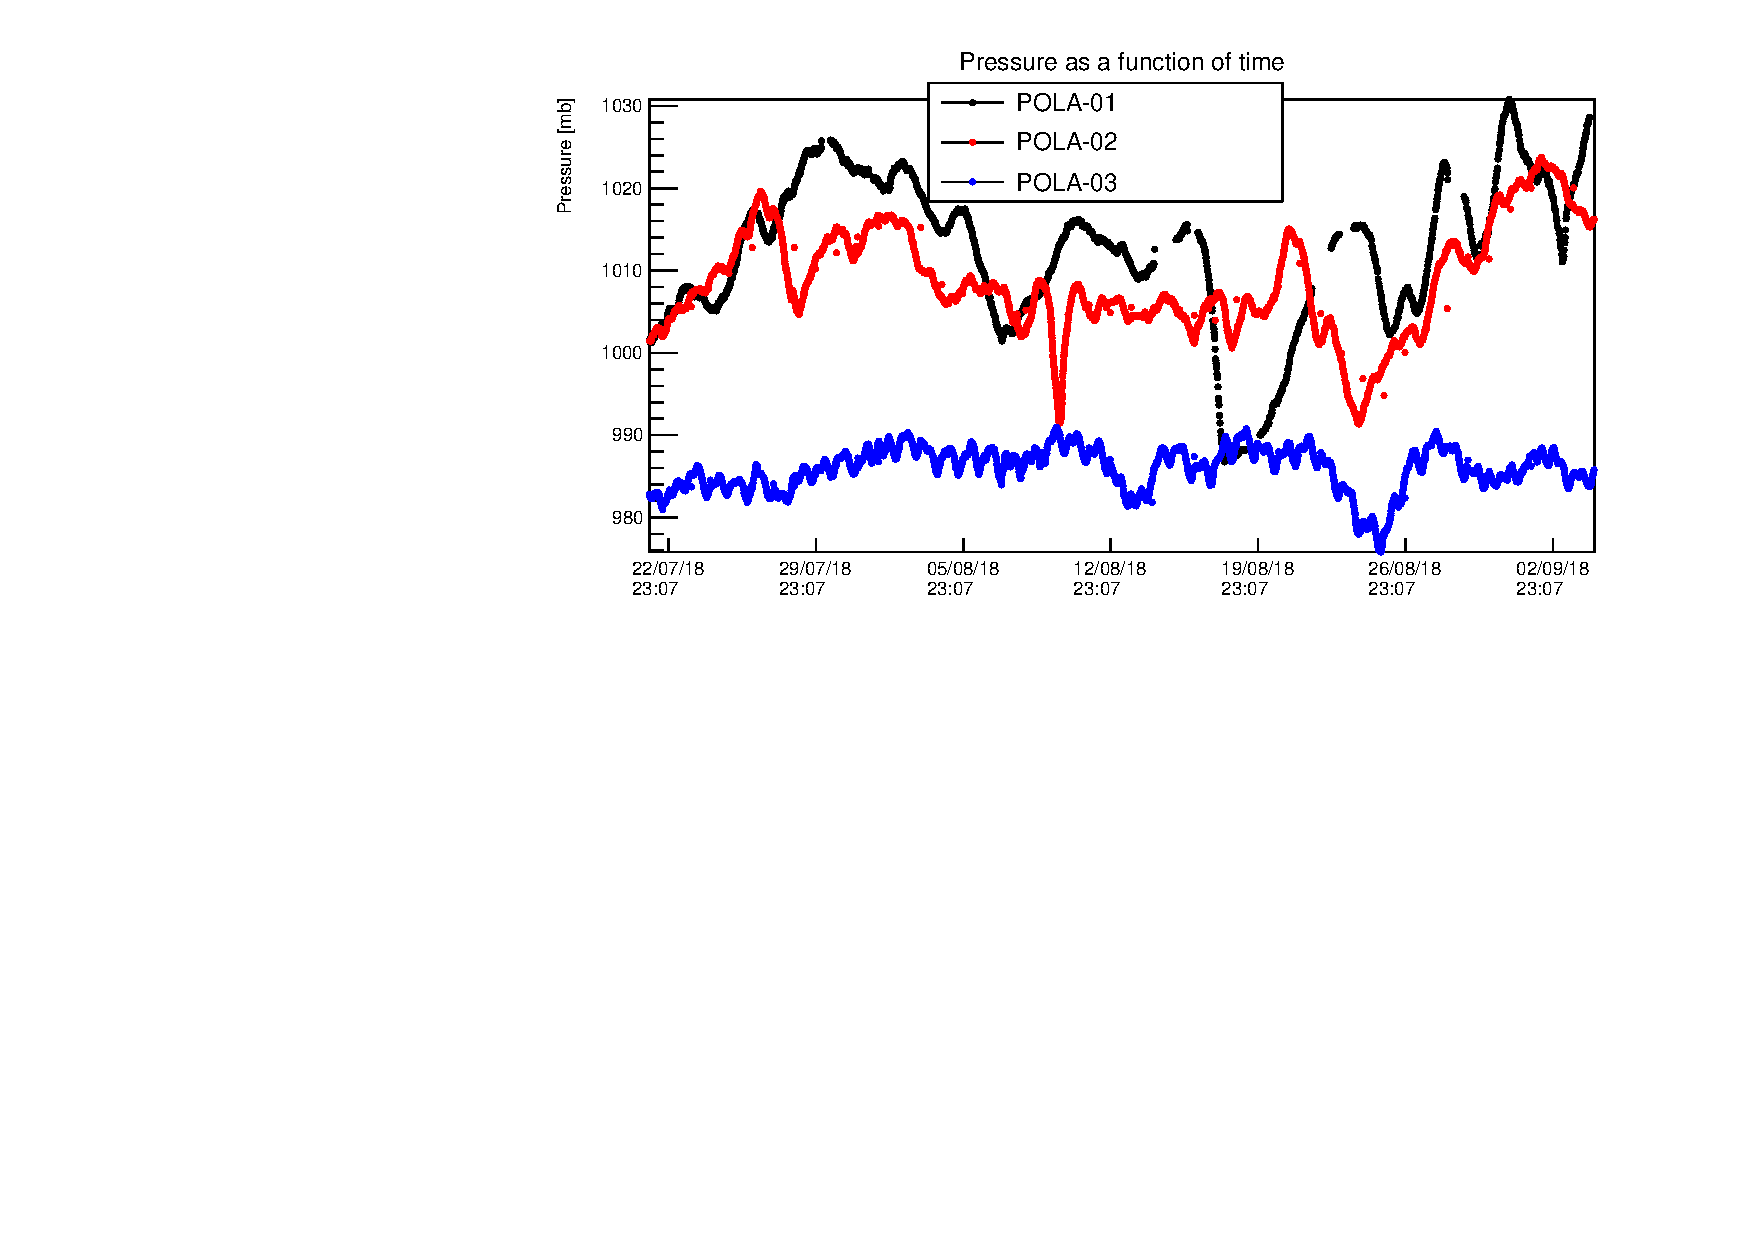
\includegraphics[width=\textwidth]{../data/plots/pressure_all.pdf}
	\caption{Barometric pressure each detector is subject to dependent on elevation above sea level.}
	\label{fig:pressure}
\end{figure}

\subsection{Particle Raw Rate}
The particle raw rate can be seen in figure~\ref{fig:RawRate}. Here, each point corresponds to a measurement of the number of events divided by time at every 12 hours. The raw rate is dependent on the atmospheric pressure, i.e. when the pressure drops there is a lower absorption of particles, thus resulting in a higher rate. The rate is also dependent on the materials surrounding the detectors. This can also be the reason why POLA-03 shows a lower raw rate compared to POLA-01 and POLA-02, because it may be surrounded by more dense materials, or be in a more compact room.

\begin{figure}
	\centering
	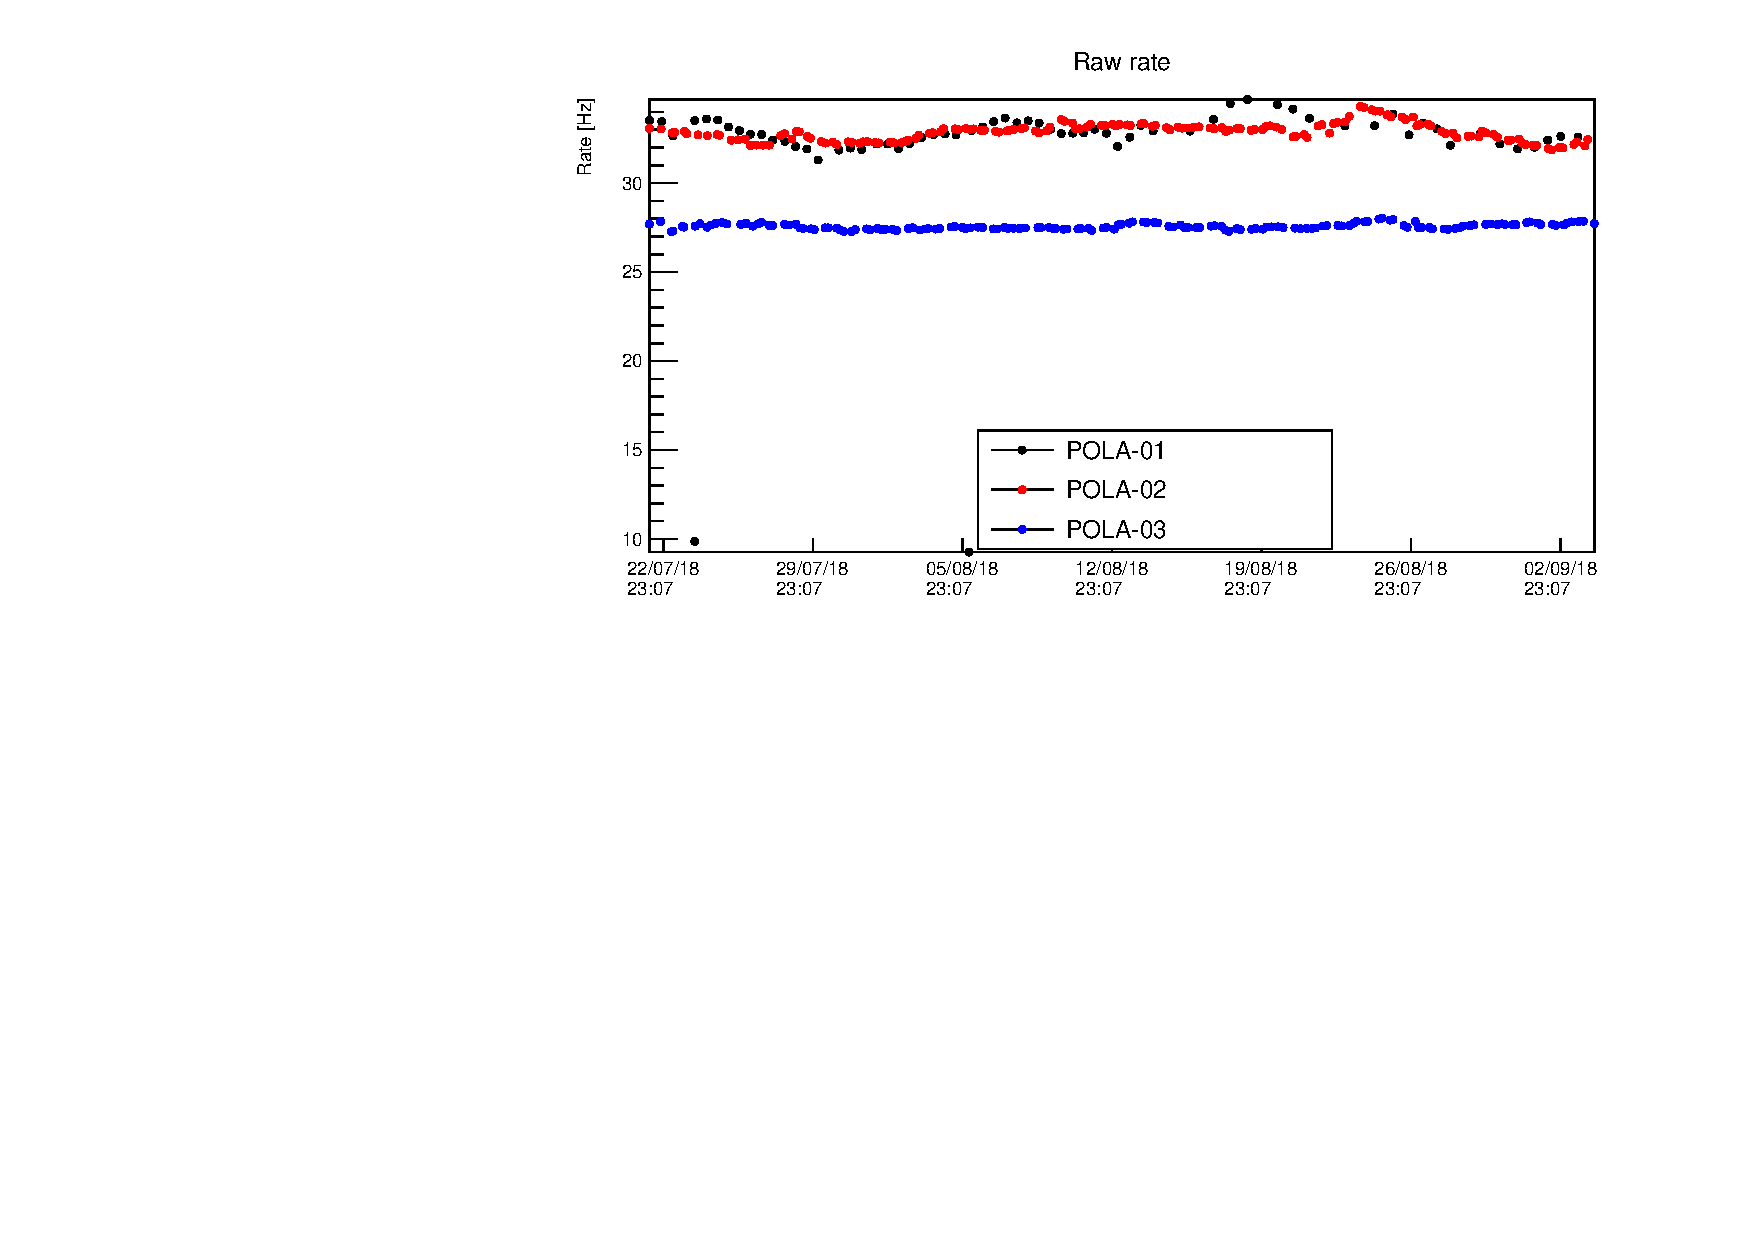
\includegraphics[width=\textwidth]{../data/plots/RawRate_all.pdf}
	\caption{Raw rate as measured by each detector.}
	\label{fig:RawRate}
\end{figure}

\subsubsection{Longitude and latitude}
The latitude and longitude for POLA-01 onboard Nanuq can be seen in figure~\ref{fig:longitude_and_latitude}. We see from figure ~\ref{fig:RawRate} that the rate is relatively flat, which is to be expected from the theory of Arthur Compton from 1933, in which the intensity of cosmic rays remains constant approximately above latitudes of $60^\circ$N. When compared to the POLA-02 as a reference point, the variations\footnote{This is performed for the raw rates of POLA-01 and POLA-02, i.e. $\sigma\left(\frac{POLA-01/\langle POLA-01\rangle}{POLA-02/\langle POLA-02 \rangle}\right)$, in which we have excluded the two outliers of figure~\ref{fig:RawRate} corresponding to values less than 10.} of the raw rate is $2.04\%$. 

\begin{figure}
\centering
	\begin{subfigure}[b]{0.6\textwidth}
	\centering
		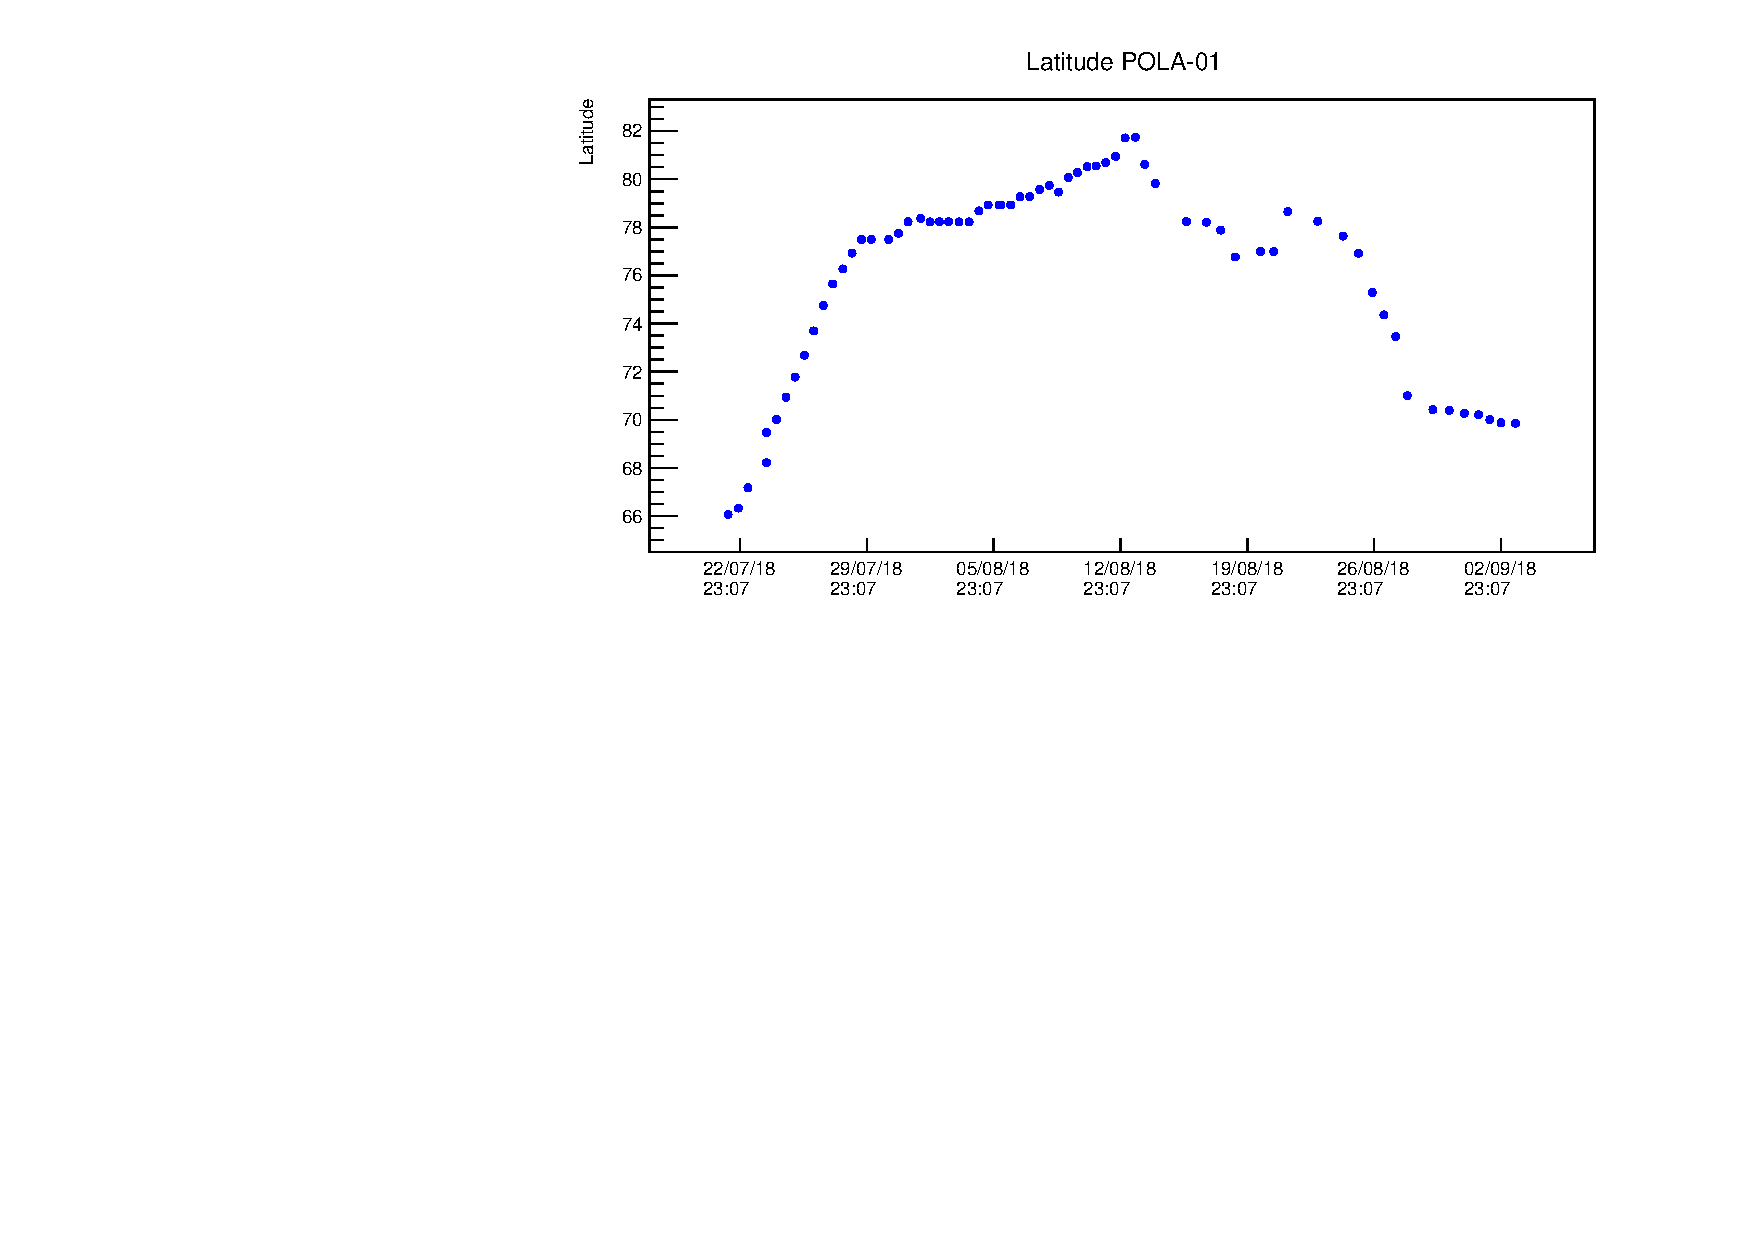
\includegraphics[width=\textwidth]{../data/plots/POLA-01/Latitude_POLA-01.pdf}
		\caption{Latitude}
		\label{fig:latitude_POLA-01}
	\end{subfigure}%
	\begin{subfigure}[b]{0.6\textwidth}
	\centering
		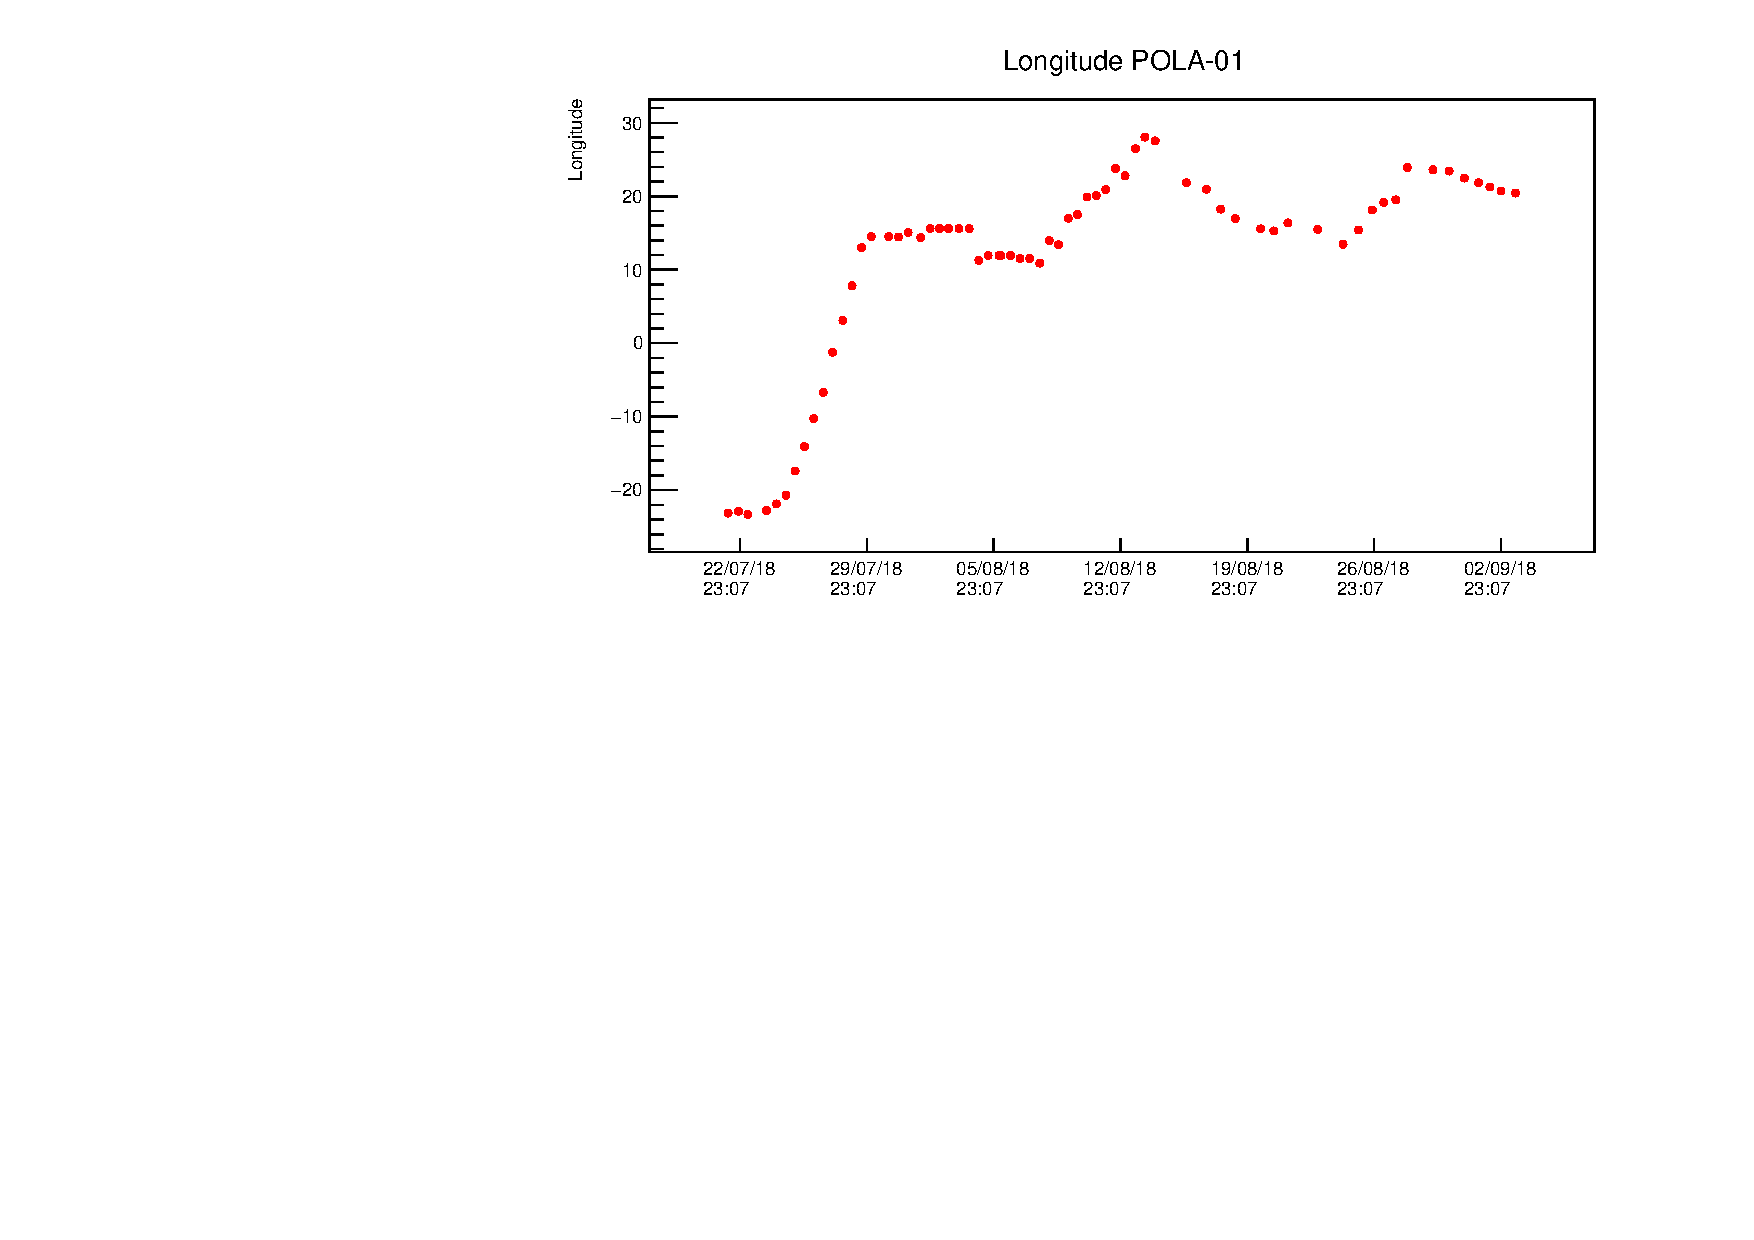
\includegraphics[width=\textwidth]{../data/plots/POLA-01/Longitude_POLA-01.pdf}
		\caption{Longitude}
		\label{fig:longitude_POLA-01}
	\end{subfigure}
	\caption{Latitude and longitude of POLA-01 measured at every 12 hours.}
	\label{fig:longitude_and_latitude}
\end{figure}


\subsubsection{Pressure and temperature}
The raw rate as a function of the pressure can be seen in figure~\ref{fig:RawRate_pressure}. Here, we see a clear distinction between the detectors. The POLA-01 and POLA-02 detectors are each subject to approximately the same pressure in which the raw rate appears to be higher than POLA-03. However, as explained above, this may be due to the materials the detector POLA-03 was surrounded by. We see however a negative gradient of the rate in all three detectors as the pressure increases, as expected. In figure~\ref{fig:RawRate_OutdoorTemp} we see that the rate remains approximately constant, i.e. independent of the temperature. The gradients of the raw rate as a function of pressure and temperature for each detector was found by linear regression and can be seen in table~\ref{tab:rawrate_gradients}. Here\footnote{The raw rate for POLA-01 has been corrected by excluding the two outliers as seen in figure~\ref{fig:RawRate}.}, the gradients of the raw rate as a function of the pressure $P$ are relatively consistent with one another confirming the statement above. However, when looking at the rate as a function of the temperature then the gradients do not appear as consistent, which may be due to lack of data included in the linear regression thus causing greater uncertainties.

\begin{table}[]
\caption{Gradients of the raw rate as a function of pressure, $P$, and outdoor temperature, $T_{out}$.}\label{tab:rawrate_gradients}
\begin{tabular}{c|cc}
\hline\hline
        & $P$        & $T_{out}$  \\ \hline
POLA-01 & -7.047e-02 & -4.307e-03 \\
POLA-02 & -6.808e-02 & 0.533      \\
POLA-03 & -4.127e-02 & 0.0610    \\
\hline \hline
\end{tabular}
\end{table}

\begin{figure}
\centering
	\begin{subfigure}[b]{0.6\textwidth}
	\centering
		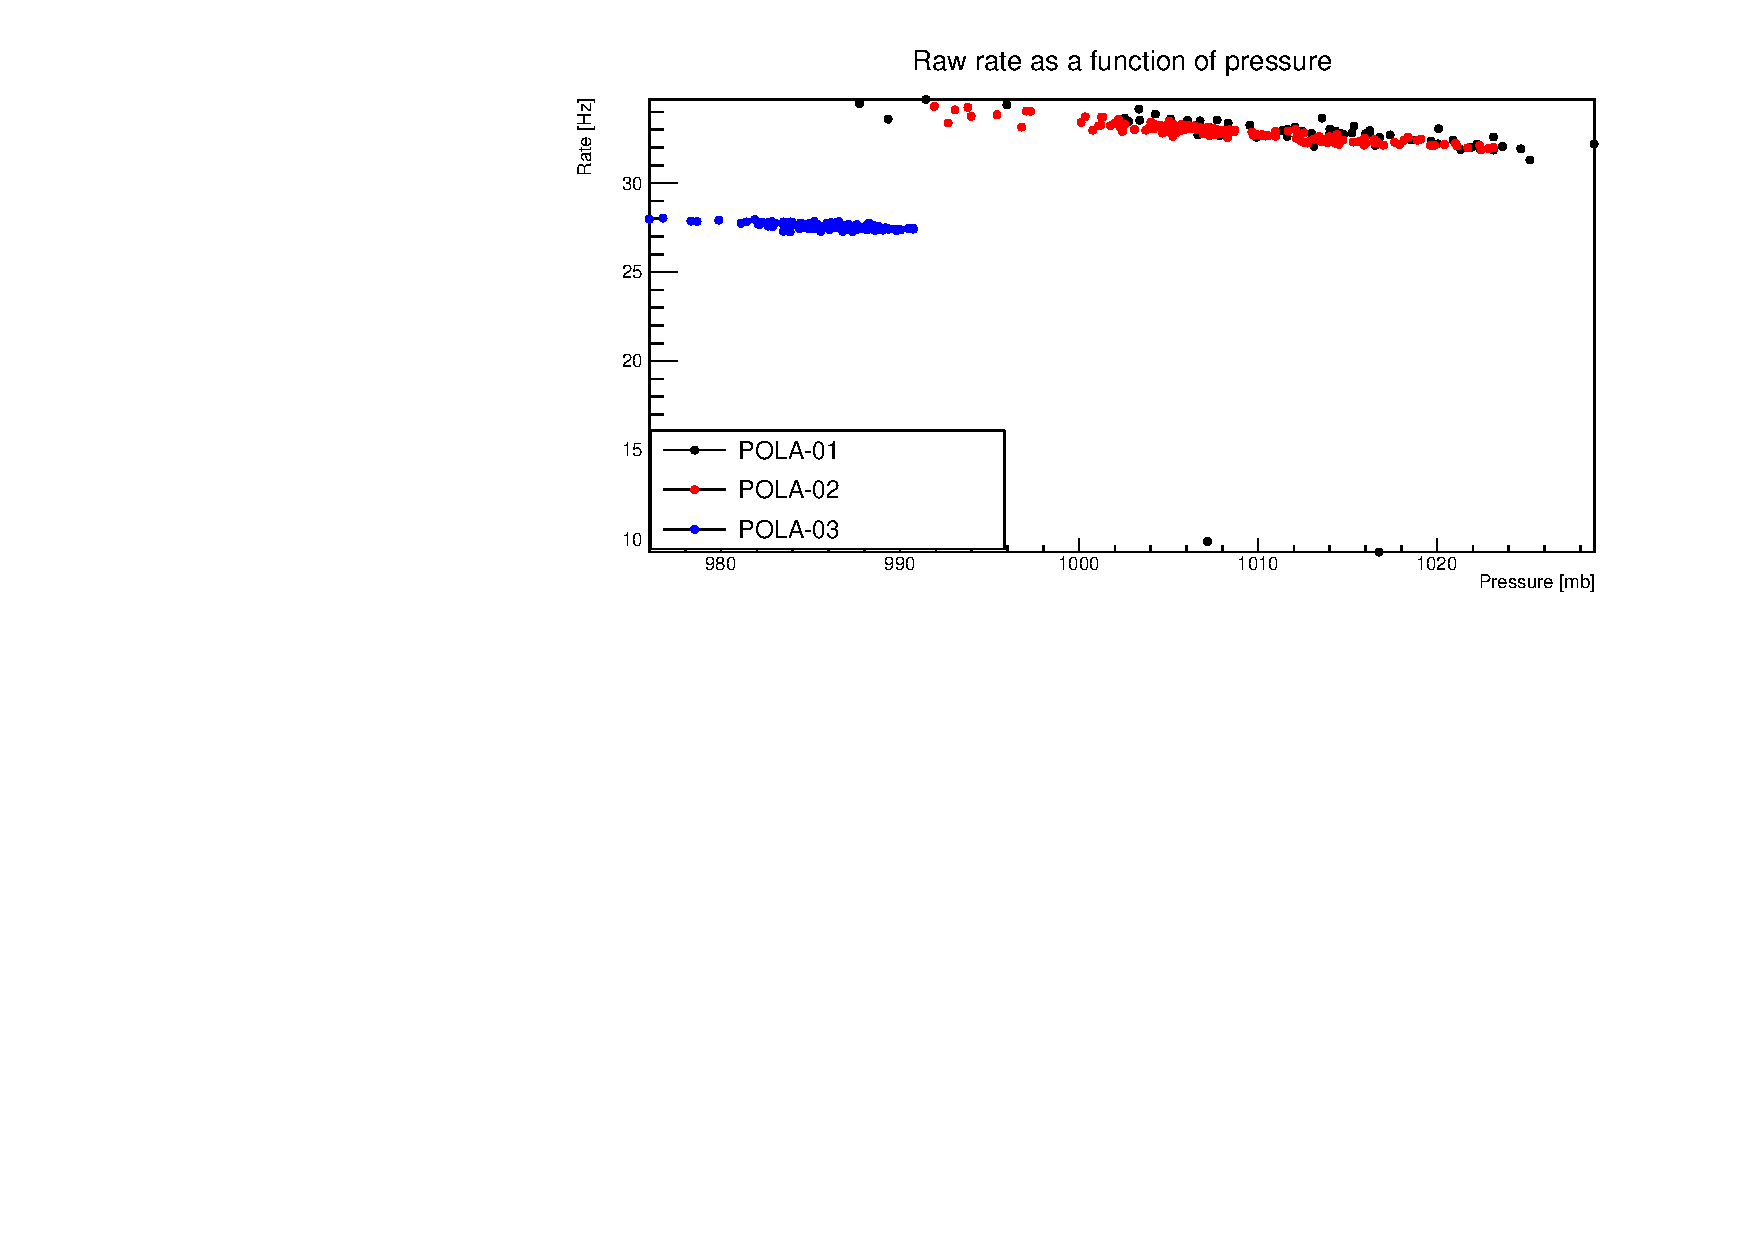
\includegraphics[width=\textwidth]{../data/plots/RawRate_pressure_all.pdf}
		\caption{Raw rate as function of pressure.}
		\label{fig:RawRate_pressure}
	\end{subfigure}%
	\begin{subfigure}[b]{0.6\textwidth}
	\centering
		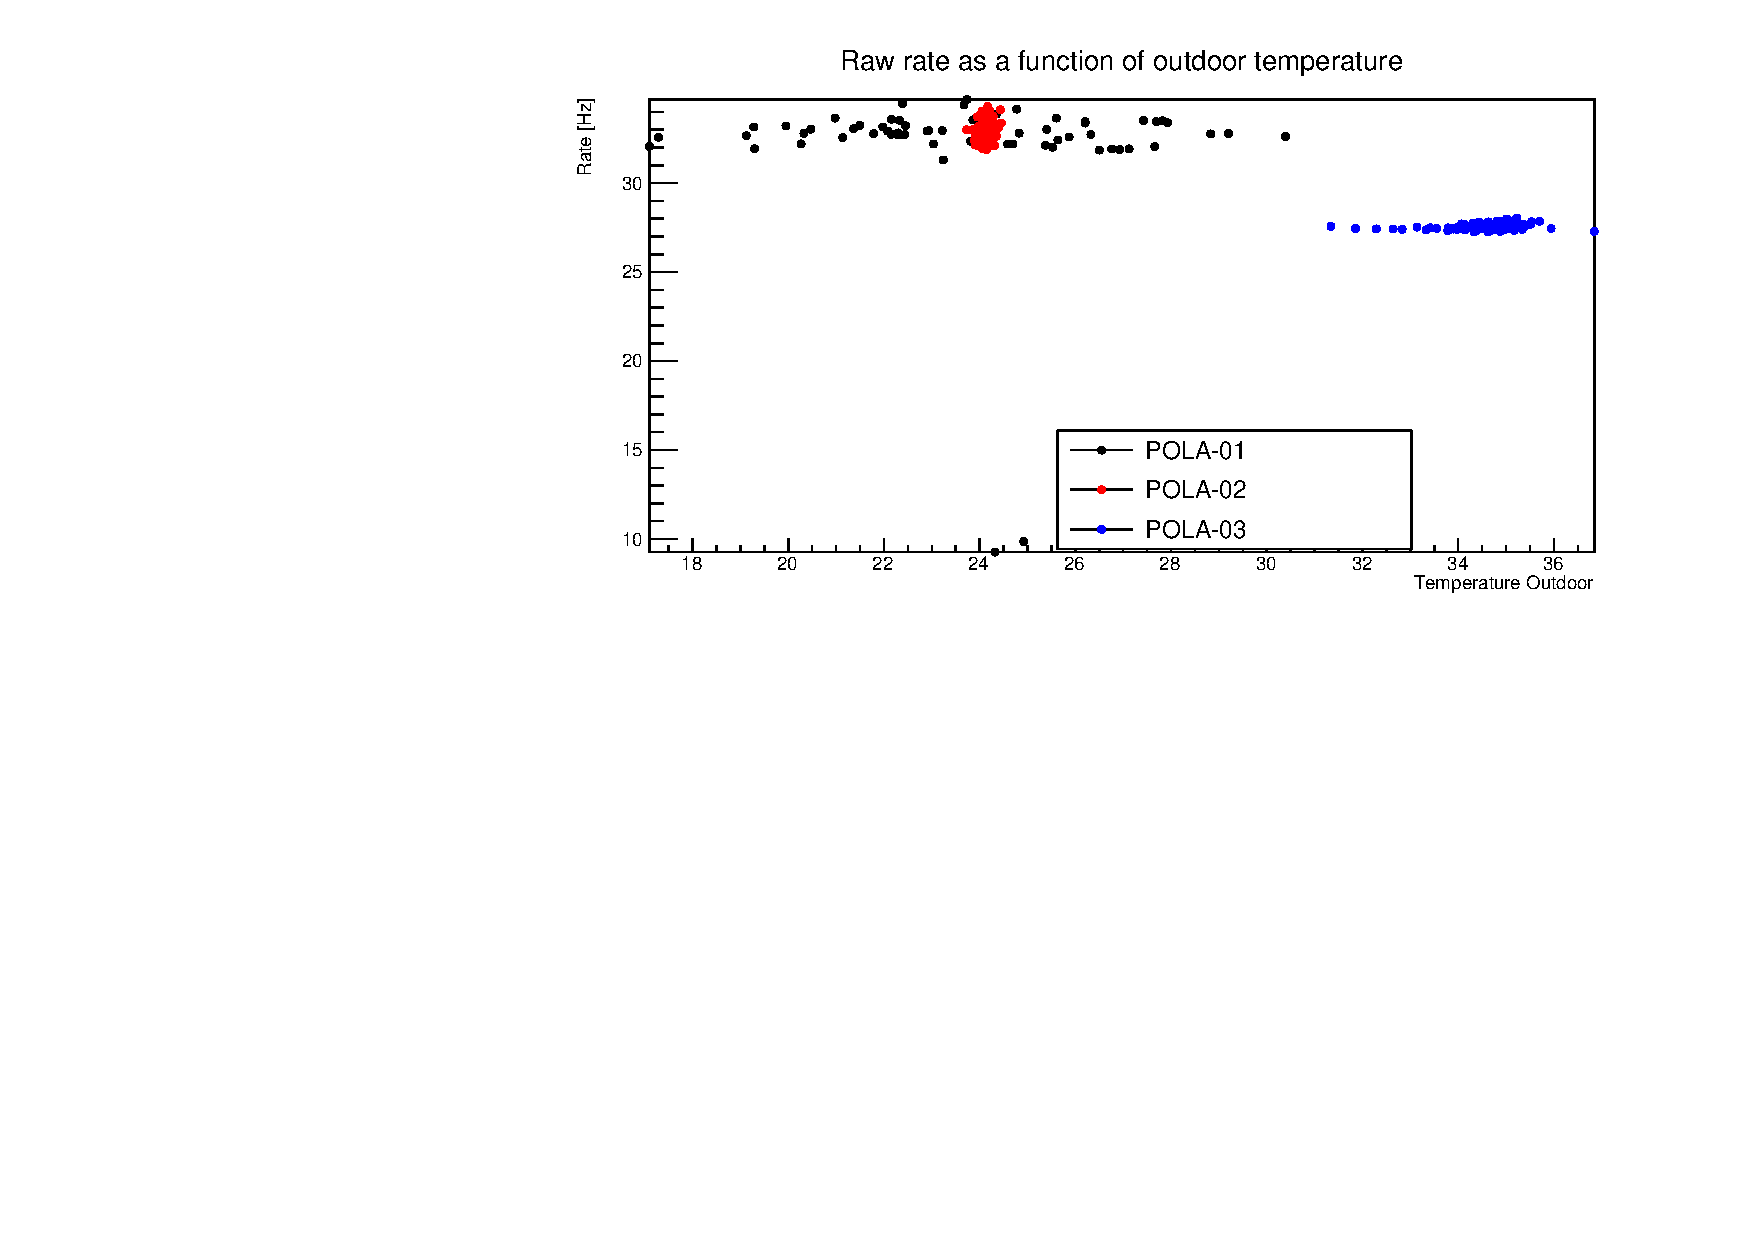
\includegraphics[width=\textwidth]{../data/plots/RawRate_OutdoorTemp_all.pdf}
		\caption{Raw rate as function of temperature.}
		\label{fig:RawRate_OutdoorTemp}
	\end{subfigure}
	\caption{Raw rate as function pressure and of the outdoor temperature close to the electronics.}
	\label{fig:rawrate_pressure_temp}
\end{figure}

\subsubsection{Corrected raw rate}
The barometric correction coefficients, $\gamma(p)$, to the raw rate can be expressed as
\begin{align}
\gamma(p) = e^{\alpha + \beta(p-p_{ref})}
\end{align}

where $\alpha$ and $\beta$ can be found by a least squares polynomial fit to the 1'st degree. In doing so we find the values as declared in table~\ref{tab:alpha_beta}.

\begin{table}[]
\caption{Values for parameters $\alpha$ and $\beta$ for the barometric correction coefficients as found by linear regression.}
\label{tab:alpha_beta}
\begin{tabular}{c|cc}
\hline\hline
        & $\alpha$ & $\beta$    \\ \hline
POLA-01 & 3.457    & -1.795e-03 \\
POLA-02 & 3.493    & -2.069e-03 \\
POLA-03 & 3.317    & -1.493e-03 \\
\hline\hline
\end{tabular}
\end{table}

In calculating the corrected rate we can divide the raw rate by the barometric corrected coefficients, in which we choose to ignore $\alpha$. This is due to the fact that $\alpha$ can still be considered a biased parameter dependent on the conditions as discussed above. The corrected rate over time can be seen in figure~\ref{fig:CorrectedRate} which, compared to figure~\ref{fig:RawRate}, displays smoother curves resulting in less variance in our dataset. As a final note, the rate for the POLA-03 detector, as explained above, lies systematically lower than that of POLA-01, and -02, which can be caused by how dense the material surrounding the detectotr is. Thus, the materials surrounding a detector can have a significant effect on the rate measured.

\begin{figure}
\centering
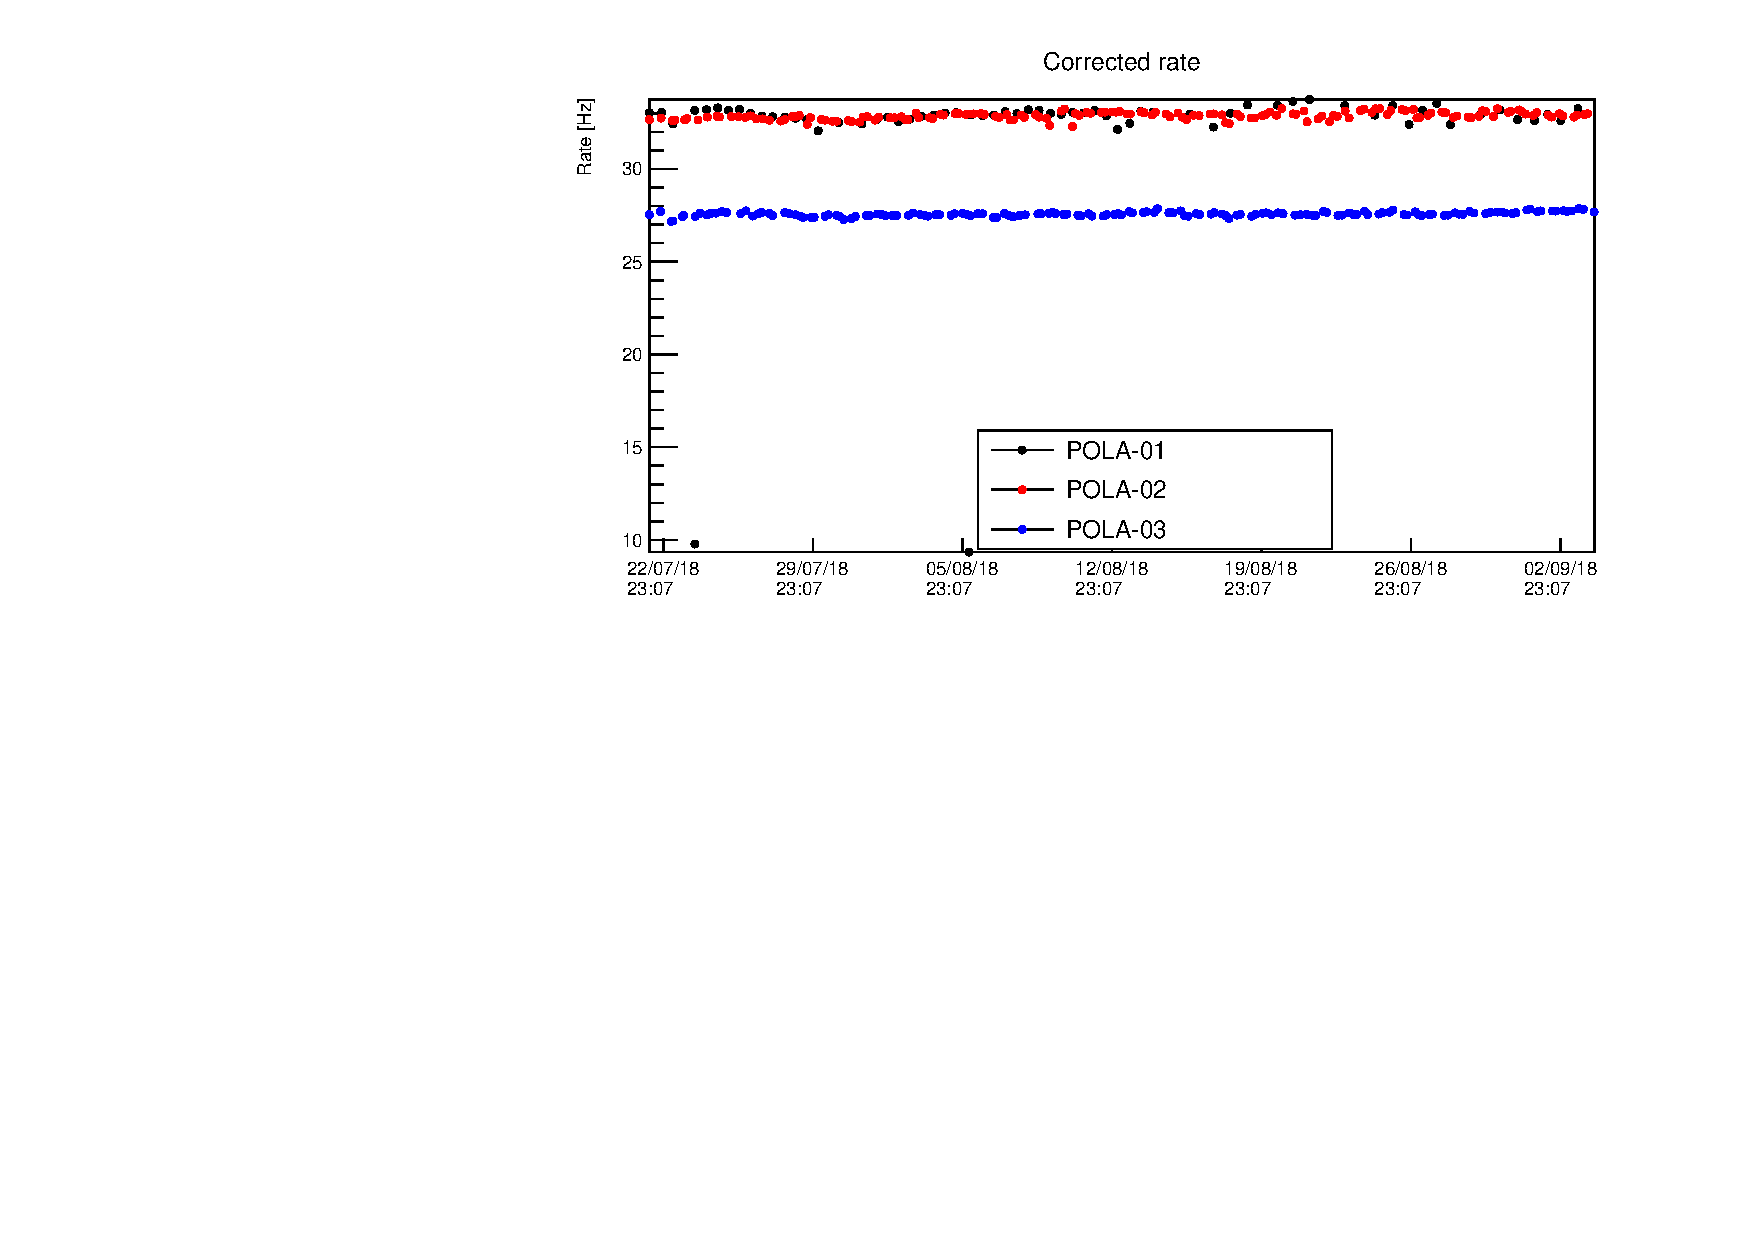
\includegraphics[width = \textwidth]{../data/plots/CorrectedRate_all.pdf}
\caption{Corrected raw rate as a function of time.}
\label{fig:CorrectedRate}
\end{figure}


\printbibliography


\end{document}









